\documentclass[english]{article}
\usepackage{amsfonts}
\usepackage{dot2texi}
\usepackage[utf8]{inputenc}
%\usepackage{babel}
\usepackage[backend=bibtex, url=false]{biblatex}
\usepackage{hyperref}
\usepackage{mathtools}
\usepackage[printonlyused]{acronym}
\usepackage{minted}
%\usepackage{amsthm}
\usepackage{amsmath}
\usepackage{tikz}
\usepackage{graphicx}
\usepackage[linesnumbered, boxed]{algorithm2e}
\usepackage{amssymb}

\usetikzlibrary{shapes,arrows}

\hypersetup{
    colorlinks,
    citecolor=black,
    filecolor=black,
    linkcolor=black,
    urlcolor=black
}

\bibliography{library.bib}

% Add mathematical foo
\newcommand{\join}{\operatorname{join}}
\newcommand{\apply}{\operatorname{apply}}
\newcommand{\eval}{\operatorname{eval}}
\newcommand{\prot}{\operatorname{prod}}
\newcommand{\quot}{\operatorname{quote}}

\newcommand{\EI}{\operatorname{EI}}
\newcommand{\normal}{\mathcal{N}}
\newcommand{\x}{\mathbf{x}}
\newcommand{\E}{\mathbb{E}}
\newcommand{\M}{\mathcal{M}}
\newcommand{\X}{\mathcal{X}}
\DeclareMathOperator*{\argmin}{arg\,min}
\DeclareMathOperator*{\argmax}{arg\,max}

\newmintinline[python]{python}{showspaces}

\begin{document}

%\title{Bayesian Optimization in Self-Referential Search Spaces}
%\author{Moritz Meier}

\begin{titlepage}
	\centering
	%\includegraphics[width=0.15\textwidth]{example-image-1x1}\par\vspace{1cm}
	{\scshape\LARGE Universität Osnabrück\par}
	\vspace{1cm}
	{\scshape\Large Master Thesis\par}
	\vspace{1.5cm}
	{\huge\bfseries Bayesian Optimization in Self-Referential Search Spaces\par}
	\vspace{2cm}
	{\Large\itshape Moritz Meier\par}
	\vfill
	First Supervisor:\par
	\textsc{Prof.~Dr.~Gordon Pipa}\par
  \vspace{1cm}
  Second Supervisor:\par
	\textsc{Prof.~Dr.~Frank Jäkel}\par
	\vfill

% Bottom of the page
	{\large \today\par}
\end{titlepage}



\begin{center}
\textbf{Declaration of Authorship}
\end{center}
I hereby certify that the work presented here is, to the best of my knowledge and belief, original and the result of my own investigations, except as acknowledged, and has not been submitted, either in part or whole, for a degree at this or any other university.


\noindent\begin{tabular}{ll}
&\\[8ex]
\makebox[2.5in]{\hrulefill} & \makebox[2.5in]{}\\
Signature & \\[8ex]% adds space between the two sets of signatures
\makebox[2.5in]{\hrulefill} & \makebox[2.5in]{}\\
City, Date & \
\end{tabular}


\newpage

\tableofcontents
\newpage


\section{Introduction}
In the past years a growing amount of collected data caused an increasing application of automated data processing in a wide range of areas streching from  science to industry.
The heigh demand of experts with an understanding of computer programming and statistical methods causes many people from other fields to expand their skill set into machine learning methods. Other than more traditional parts of software engeneering, machine learning is still in the process of finding efficient workflow standards. More and more data processing software libraries targeting different aspects of machine learning application are released. Especially the need for easy-to-use / out-of-the-box let to high-level led to interfaces that implement aspects of declarative model design. The dataflow processing computation model turned out especially suited for data processing. In the deep learning field libraries like Theano and Tensorflow allow the user to construct computation graphs, which are automatically optimized and compiled into efficient machine code.

\begin{figure}[h]
  \centering
  \includegraphics[scale=0.7]{figures/ml-workflow.pdf}
  \caption{Simplified overview of a machine learning workflow.}
  \label{ml-workflow}
\end{figure}

Figure \ref{ml-workflow} shows a simlified view of a machine learning workflow. First an algorithm is selected, which is trained to obtain a model. The model is validated to measure generalization. This process is repeated for different algorithms, until a satisfying performance is reached, or a time limit is exceeded. This selection procedure, which is not considered as training in the previous overview, is the subject of research in this these.
The selection is usually a two step process: First from the range of aplicable machine learning algorithms the most promising one is selected. This step is nearly always done manually. In a second step the algorithm configuration is chosen. This selection problem is addressed in the field of hyperparameter optimization.
Hyperparamter optimization problems are usually black-box optimization problems, since less or nothing is known about the function. Furthermore the  landscape is often multimodal and sometimes discontinous. The especially nasty nature of this problem leads to a frequent usage of naive methods, like random or exhaustive search.
In black-bock optimization the only source of information about the objective function, is the evaluation of the objective function itself. Model-based global optimization methods try to harness this information by estimatating the objection function, allowing to make predictions for unknown points. In this way the number of function evaluations should be kept low (since this is the costly step), while the amount of information about the objective function, especially good performing areas, which is obtained in the process should be maximized.
In recent years Bayesian optimization as a method for hyperparameter optimization received some attention. A Bayesain model of the objective function, which essential means to have a distribution over function values, enabled to express the trade of between exploration and exploitation as a form of inference.
Hyperparamter optimization can be extendet to a simultanious selection of algorithm and configuration. This problem is formally defined in \cite{feurer_efficient_2015} as the Combined Algorithm Selection and Hyperparameter optimization problem \textit{CASH} and belogs to the field of \textit{automated machine learning}. The configuration space varies among different algorithms, such that the relevance of a certain parameter depends on the selected algorithm. The Tree-Parzen-Estimator and SMAC have been developed to deal with this conditional parameters.
Going a step further the parameter space can become even more complicated. If one considers for example multilayer perceptrons, where the number of layers needs to be chosen before the number of neurons per layer. In this case the number of model paramters can be of arbitray number. Another example is the space choice of a kernel in a support vector machine or a Gaussian process regression, where the combination of kernels is defined by a grammar of base kerels and kernel combinations.
This work proposes a formalism to state optimization problems by describing the structure of search spaces together with a distribution over the values. The search spaces can range from simple one-dimensional or multi-dimensional strucutres, over spaces that comprise multiple algorithms and their hyperparameters to complicated infinte grammar based structures. This is achieved by allowing to add expressions that refere to the search space itself. The language is comparable to the computation graph construction in Theano with the ability to formulate sets or distribtuions of computation trees. The syntax is related to a language for hyperparameter optimization problem description described in \cite{bergstra_making_2013} which was also used for the hyperopt libray \cite{bergstra_hyperopt:_2013}. The second contribution is an algorithm that extends known Bayesian optimization algorithm, such that optimizations on self-referential search space descriptions can be conducted. The algorithms is effectively a solver for problems stated in the language.
Section 2 discusses the probelm of global black-box optimization in general. Section 3 narrows the view point to hyperparamter optimization.
Section 4 shortly introduces Gaussian process regression, since they are from the Bayesian model in the algorithms.
Section 5 explains methods of Bayesian optimization.
Section 6 describes the search space description formalism.
Finally section 7 exmplains the tree Bayesian algorithm.
Section 8 give some comments to the implementation and show code examples.
In Section 9 the results of a row of experiments that apply the system to various differnt problems is presented.

\newpage

\section{Hyperparameter Optimization}
In Bayesain statistics the term \textit{hyperparameter} referes to a parameter of the prior distribution. In \textit{hierarchical models} the prior distribution over the hyperparamters are called \textit{hyperpriors} respectively \cite[p.408]{bishop_neural_1995}. In ML a hyperparameter is any parameter that needs to be assigned before the training of other parameters can begin. The ML definition is adopted here. The selection procedure usually involves repetitive training of ML-algorithm with various hyperparameter combinations and rating by some quality measure. This nesting gives rise to an alternative label for hyperparameters as \textit{outer loop} in contrast to \textit{inner loop} parameters that are selected by the ML-algorithm itself. Other terms for HPO are hyperarameter \textit{search} or \textit{tuning}.
Also \textit{model selection} means essentially the same thing, the focus is however more on the selection criterions.

Despite decades of research in global optimization the predominant methods for HPO are of modest complexity. A review of all 86 papers from the NIPS2014 conference revealed that the fast majority used either grid search or default parameters\footnote{\url{http://github.com/jaak-s/nips2014-survey}}. Grid search (sometime also "parameter scan"), is an exhaustive search over a predefined subset of the full parameter space. The points have equal distance within one input dimension forming the interjections of a grid, whereby all kind of varaition is possible in the placements. In contrast the random search picks samples from a distribution over the parameter space (mostly uniform distribution). Both methods are unadaptive in the way that the next parameter setting $\lambda$ is independent of any previous evaluation. A combination of one of these methods together with random search is also popular. A reasons for this preference is that both algorithms are trivial to implement and parallelize. A recent comparison between random and grid search has shown that random search is empirically and theoretically superior \cite{bergstra_random_2012}. This result is explained by the  \textit{low effective dimension} of the parameter space. Intuitively that means that the value of certain parameters can become irrelevant if other parameters have a certain allocation. In grid search all settings of an ineffective parameter are evalutated while the rest of the parameters are constant in each step. In random search all parameters change all the time, such that an optimization with an ineffective parameter is equivalent to a lower dimensional optimization with this parameter fixed.

\subsection{Global Optimization}
Optimization problems occur in a wide range of fields in various different forms. There are different fields that are solely concerned with optimization problems of one kind or another. \textit{Mathematical programming} is the subbrach of applied mathematics, that is concerned with optimization. Classes of problems are stated formally, ofter together with with additional eqaulity or inequality contraints. The solution (algorithm) comes usually with a formal proofs of convergence or accurracy bounds. The field of \textit{Metaheuristics}
on the other side is rather based on intuitions, metaphoric priniciples and validation by simulation. A metaheuristic can be defined as "a high-level problem-independent algorithmic framework that provides a set of guidelines or strategies to develop heuristic optimization algorithms". \cite{sorensen_history_2014} Due to generality in method and application of the field, a vast amount of algorithms that are tageted to global optimization, led to a confusing (almost litteral) \textit{zoo of metaheuristics}. Researches with sometimes minor mathematical background, adopted metaphors from other scientific fields to describe algorithms in unconentional terminology which obscurify the relations to more established methods. \cite{sorensen_metaheuristics-metaphor_2015}


On the most general level optimization algorithms are devidable by some rough distincions:

\begin{itemize}
  \item \textit{Local} optimization as opposed to \textit{global} optimization just aim to find local minimas. A local algorithm can be the basis of a global algorithm, for example with local optimization from different starting points. Most optimization problems in machine learning are local, since successful algorithms are usually designed that the parameter space is convex and can be minimizes efficiently.

  \item An algorithm which makes use of the first derivative of the objective function is called \textit{gradient based} or a first order method. Algorithms that make use of the second derivative are called second order method. Famous examples are Gradient descent or newton method.

  \item If an optimization method involves random sampling at some point it is called \textit{stochastic} and \textit{deterministic} if not. This must be distinguished from \textit{probabilistic} methods that used probability theory but are usually deterministic. In the metaheuristics community the terms "heuristic" is roughly used for "stochastic" and "exact" for deterministic. Whereby the field of origin (metaheuristics or mathematics) is also a factor in the  word usage.

  \item More sophisticated \ac{GO} algorithms than random search or grid search can be devided into model-based or instance-based (a.k.a. model-free or direct) methods. Instance based methods usually population vs. single instance Population based methods remember multiple isntances.

  \item While most optimization problems in research are single-objective, in fields like eoconomics or operation research multi-objective optimizations are targeted. In this problems multiple pareto optimimal sultions can occur.

  \item Somtimes the objective function can be stochastic. Usually this happens when there is a true underlying function but the measurement of this function is distorted by noise. In hyperparameter optimization it very common that the objective algorithm is stochastic (e.g MCMC-algorithms).

\end{itemize}



\subsection{Bandit Problems}
Hyperparameter optimization falls into the class of multiarmed-bandit problems. The name makes use of a metaphor, where a gambler is faced to choose a lever from $n$ different one-armed bandits. The goal is to maximize the profit (or minimize the losses) by trading off exploration (trying new levers) and exploitation (playing at the most profitable machine). Applied to the hyperparameter problem, a parameter configuration takes the role of a lever from the metaphor. For parameter spaces comming from a real domain (or other infinte spaces) the problem is also called \textit{infinite bandit problem}.

%sequential decision making with limited information
%stationary bandit


\subsection{Active Learning \& Experimental design}
Active learning is a related method, that is applied for classification task with lots of unlabeld data which, which are expensive to label. It is very similar to BO in the way that promising unlabeld datapoint are selected by a model, which is adapted to every new label. Differences are tha labels are delivered by a human (called the \textit{oracle}) and that the samples come usually from a finite set (\textit{pool based sampling}) \cite{settles_active_2010}.

 - optimal experimental design
 - response surface model

\subsection{Machine Learning as Optimization}
Most \acf{ML} problems are expressable as optimization problems \cite{bennett_interplay_2006}. Training algorithms are (usually) derived by solving the minimization problem of some error or energy function or maximization of fittnes or utility function. From this perspective learning on the most general level can be stated as a global black-box optimization problem problem.
$$\x^* = \argmin_{\x \in \mathcal{X}} f(\x)$$
A best general solution of this problem does of cause not exists. Due to \textit{No Free Lunch} theorem for optimization, which roughly speaking states that the average performance of any algorithm across all possible optimizaion problems is identical. In other words efficient optimization without any assumptions or prior over the hypothesis space is impossible. Luckily in most cases the assumption can be made that points which are close in the input space are probabliy also close their performance. This requires a topology (structure) of the search space, which is naturally given for numerical inputs.

In his famous \textit{Statistical Learning Theory}, Vladimir Vapnik states the \textit{General Setting of the Learning Problem} as a minimization of the risk function \cite{vapnik_overview_1999}.
\begin{equation}
R(\alpha) = \int Q(z,\alpha)dP(z)
\label{risk}
\end{equation}
The risk $R$ takes the role of the objective function. $P$ is the true probability distribution over the data. The function $Q$, which is parametrized by $alpha$, measures the performance on a single data point $z$. The structure of $Q$ is left open and incorporates a possible model, algorithm or loss function. While this genral risk function is not as general as the name may suggest it still covers a majority of problems in machine learning. Since $P$ is usually unknown and represented by samples as the data, it is estimated by the more practical empirical risk function.
\begin{equation}
R_{emp}(\alpha) = \frac{1}{l} \sum_{i=1}^l Q(z_i,\alpha)
\label{empirical risk}
\end{equation}
Depending on the problem the function $Q$ takes different forms. For supervised learning, for example, a data point $z$ is a tuple of a dependent and an independent variable $(x,y)$. The task is to find a function $f$ that maps from $x$ to $y$. Eventually $Q$ can be written in terms of a lossfunction $L(y,f(x,\alpha))$.
To make it even more specific the function $f$ is actually the result of a learning algorithm $\mathcal{A}$, which can be seen as a functor mapping hyperparameter setting $\lambda$ and a training set $X_{train}$ into the hypothesis space. This leads to the definition of the hyperparamter problem as it is defined by Bergstra et al. in \cite{bergstra_random_2012}.
\begin{equation}
\lambda^{(*)} = \argmin_{\lambda \in \Lambda} \E_{\x \sim \mathcal{G}_\x}\big[\mathcal{L}\big(\x;\mathcal{A}_\lambda(X_{train})\big)\big]
\label{hypa_opt_1}
\end{equation}
Equation \ref{hypa_opt_1} is a special case of the risk function, with $Q = \mathcal{L}$ and $\alpha$ the fitted model. Note that $X_{train}$ is not requiered to be sampled form $G_x$, and thus covers learning problems where the data is separated in training and application is different.
In order to avoid overfitting and estimate the generalization error, model selection technics are applied. In special cases measures which trade off number of parameter and sample size with the training loss (like BIC or AIC) can be applied. In most practical application however, having a separated training and validation set is most popular. The empirical risc version of the hyperparmeter optimization looks like this:
\begin{equation}
  \Psi(\lambda) = \sum_{x \in X_{val}} \mathcal{L}\big(x;\mathcal{A}_\lambda(X_{train})\big)
\end{equation}
This form of the objective function also called respond function in the experiment design litterature. In most cases an exhaustive search over the whole parameter space is infeasible. The search is thus limited to a finite subset $\{\lambda_1, \lambda_2, ... \} \subset \Lambda$:
\begin{equation}
  \hat{\lambda} = \argmin_{\lambda \in \{\lambda_1, \lambda_2, ... \}} \Psi(\lambda)
\label{empirical hypa_opt_1}
\end{equation}
Now we have a practical definition of hyperparamter optimization.
% risk with loss function
%\begin{equation}
%R(\alpha) = \int L(y,f(x,\alpha))dP(x,y)
%\end{equation}

\subsection{Properties of HPO}
HPO problems have some properties that distinguishes them from other black-box optimization problems.

Training of machine learning algorithms can take minutes, hours, days or more. The costlier an evaluation is, the less evaluations are available within fixed time boundaries. Indeed the performance of an HPO algorithms can almost solely measured by the number of evaluations it takes to find values close to the optimum or reverse the best value after a fixed number of iterations. Most global optimization algorithms relay on a high amount of evaluations, which makes them unfit for HPO. The longer an evaluation takes the more time can be spend on inferring the next optimal evaluation point. So there is a tradeoff between intelligent selection and massive sampling. The evaluation time can also vary for different parameter settings. Consider the number of neurons in a neural network. More neurons take obviously longer to train than fiewer neurons.
As for other black-box optimization problems there is littel knowledge about the search space. But HPO problems go even further in the way that the parameter domains can have very different structure. Search spaces range from simple homogenic cartesian search spaces to heterogenic graph shaped spaces, with mixtures of real, integer or categorical valued paramerters. While \ac{ML}-algorithms are usually defined in a way that inner loop parameters can be optimized efficiently, usually with a convex search space, HPO spaces have no such design benefits.

On top of that a (perfect) hyperparameter optimization algorithm is faced with other affordences. First of all multicore processors and computer clusters are avaiable for most researchers nowadays. This requires an optimization algorithm to be parallelizable. Secondly a long optimization might not be a linear process and may require an interruption and a storage to disc, that can be restored for later continuation. Also the knowledge about the problem can change outside the optimization process. An algorithm that allows the interactive integration of new knowledge, maybe in the form of hints for good regions, is desirable.
At last even if one can only make a few or no assumptions about the structure of a hyperparamter search space, one has always the option to use estimations to gather information about the function faster. Many machine learning processes are iterative, so an estimation by \textit{early stopping} is possible. It is also possible to make an estimation by using only a subset of the data. If preknowledge about an algorithm is available, is the convergence behavior for more iterations can be extrapolated.
% \paragraph{scalability}
% \subsection*{computational costs}
% - space \& time
% - intelligent selection vs massive sampling tradeoff



\section{Gaussian Processes Regression}
\label{GPR}
Regression is the problem of estimating the relationship between an indendent random variable $X$ and a real-valued dependent random variable $Y$, by generalizing from examples. In frequentist settings one ususally defines a parametrized familiy of underlying functions. A point estimator is then applied to find the set of parameters that explains/predicts the data the best. In the famous maximum likelihood approach the conditional likelihood of the data $P(Y|X)$ is maximized over the model parameters. The semi-Bayesian maximum a posteriori approach additionally assumes a prior probability over the model-parameters and can e.g. deal with overfitting in a natural way. Finally in the fully Bayesian approach the estimates are distributions over parameters rather than single paramters settings. Gaussian process regression goes even a step further by having a non-parameteric model that grows with in complexity with the amount of data (Some authers prefere to call them inifinte-parametric models for that reason).

A Gaussian process (GP) is a (usually infinite) collection of random variables where any finite subset is multivariat normal distributed. These random variables can be indexed by $\mathbf{x} \in \mathbb{R}^n$, such that the GP can be seen as a distribution over functions $\mathbb{R}^n \rightarrow \mathbb{R}, x \mapsto f(\mathbf{x})$. This is written like:
$$f(\mathbf{x}) \sim \mathcal{GP}\big(m(\mathbf{x}), \kappa(\mathbf{x},\mathbf{x}')\big)$$
Where $m$ is the function of the expected value, and $\kappa$ the covariance function or kernel. The kernel determines the covariance between two function outputs in dependence of function inputs.
$$\kappa(\mathbf{x},\mathbf{x}') = \operatorname{cov}(f(\mathbf{x}),f(\mathbf{x}'))$$
In order to sample from the prior the multvariat normal distribution can be used. The sample points $X_*$ are applied to the kernel to get the covariance matrix $K_{**} = \kappa(X_*,X_*)$. For comptational simplicity the prior mean is usually set to $m(\mathbf{x}) = \mathbf{0}$.
$$\mathbf{f_*} \sim \mathcal{N}(\mathbf{\mathbf{\mu}}, K_{**})$$
Samples for different covariance functions can be seen in figure \ref{kernels}.

The key to use Gaussian processes for regression is the conditional distribution of unseen points in dependence of already observed points.
To obtain the conditional distribution, the joined distribution is formulated first.

$$
\begin{bmatrix}
\ \mathbf{y}\ \\
\ \mathbf{f_*} \\
\end{bmatrix}
\sim \mathcal{N} \Bigg(\mathbf{0},
\begin{bmatrix}
K_y & K_* \\
\ K^{\top}_{*} & K_{**}  \\
\end{bmatrix}
\Bigg)
$$
$K_y$ is the covariance matrix for some hyopthetical input points. $K_*$ is the covariance of matrix of the observed and unobserved points. All four matricies together form a big covariance matrix for the joined distribution. Next the usual formula to condition a normal distribution on some variables is applied, to obtain the predictive distribution.
$$\overline{\mathbf{f_*}} = K_*^\top K_y^{-1}\mathbf{y}$$
$$cov(\mathbf{f_*}) = K_{**} - K_*^\top K_y^{-1} K_*$$
The mean posterior $\overline{\mathbf{f_*}}$ and convariance $cov(\mathbf{f_*})$ fully determines the posterior distribution for the predicted points. For interpolation (noise free prediction) $K_y$ is set to  $\kappa(X,X)$. For noisy prediction $K_y$ gets an additional noise term $\kappa(X,X) + \sigma_n^2I$. Figure \ref{gpr} shows a posterior distribution with and without noise.

\begin{figure}

  %\begin{minipage}{0.5\textwidth}
  %\includegraphics[scale=0.3]{figures/prior_plot.pdf}
  %\end{minipage}%
  \begin{minipage}{0.5\textwidth}
  \includegraphics[scale=0.3]{figures/posterior_no_noise.pdf}
  \end{minipage}%
  \begin{minipage}{0.5\textwidth}
  \includegraphics[scale=0.3]{figures/posterior_with_noise.pdf}
  \end{minipage}%
  %\begin{minipage}{0.5\textwidth}
  %\includegraphics[scale=0.3]{figures/posterior_exp.pdf}
  %\end{minipage}%

  \caption{Left: Posterior for some sample points, without noise term. The blue area displays the margin of the variance. The variance is zero for observed points. Right: Posterior with noise term. Observed points have non-zero but reduced variance.}
  \label{gpr}
\end{figure}


Note that even though the model is a Gaussian process, the calculations can be done with mutivaraite Gaussian distributions and have a time complexity of only $O(N^3)$.

The actual implementation of \ac{GPR} requires further knowledge about numeric properties which are not discussed here. A practical algortihm description involving Cholesky decomposition can be found in \cite[Algorithm 2.1]{rasmussen_gaussian_2006}.




\subsection{Covariance Functions}
With the choice of the kernel function the generalization behavior can be modulated.  A property of most kernels in use is \textit{stationarity}. A stationary kernel can be written as a function of $\x-\x'$ and is hence a tanslation invariant function.

A quadratic matrix $K$ with $\mathbf{v}^\top \mathbf{v} \ge 0$ for all $\mathbf{v} \in \mathbb{R}^n$.

The \textbf{squared-exponential} kernel (SE), which is also called radial basis function kernel (RBF), has many desireble properties. For closer points the correlation tends towards one, while the correlation of farer points tends towards zero. This leads to very smooth function.
$$\kappa_{se}(x, x') = exp\bigg(-\frac{(x-x')^2}{2\ell^2}\bigg)$$
The two parameters varaince $sigma^2$ and lengthscale $\ell$ occur in many kernels.

With the \textit{periodical} kernel stationary periodical pattern can be fitted.
$$\kappa_{per}(\x,\x') = \sigma^2exp\bigg(-\frac{2 \sin^2(\pi|x-x'|/p)}{\ell^2}\bigg)$$
The \textit{exponential} kernel produces continous but non-differential functions.
$$\kappa_{exp}(\x,\x') = exp\bigg(-\frac{|x-x'|}{\ell}\bigg)$$
The \textbf{linear} kernel is non-stationary.
$$\kappa_{lin}(x, x') = \sigma^2 + \x\cdot\x'$$
GPR with a linear kernel is Bayesian linear regression.
The kernel parameter can be varied in order to improve the datafit. These parameters are usually ajusted by optimizing the marginal likelihood.

\paragraph{Kernel Composition}
Kernels can be combined in order to gain new kernels, which inherits properties of both base kernels. The product of two linear kernels for example will assume a quadratic trend in the data. The local periodic kernel is the product of the periodic and the RBF kernel.

\paragraph{Non-Continous Variables}
It is possible to define meaningfull kernels for all kinds of  non-continous variables. For interger valued variables the same kernels still be used. For nominal scaled variables a euclidian distance variable values cannot be assumend any more. A kernel especially for categorical variables is described in \cite{hutter_sequential_2011}. It is based on the hamming distance, which is known from coding theory and counts the common digits of a bitstring. A simple trick to use the kernels for continous variables on categorical ones is to use a one-hot coding on the categories together with a RBF kernel. Each category is map in a new dimension. This approach can be problematic for a big amount of categorical values, since optimization and prediction can become costlier.

\begin{figure}
  \includegraphics[width=1\textwidth]{figures/kernels_and_samples.pdf}
  \caption{The upper row are the convariance functions. The lower row the corresponding samples from the prior distribution.}
  \label{kernels}
\end{figure}

\newpage


\section{Bayesian Optimization}
Bayesian optimization (BO) is model-based black-box optimization with a probabilistic model for the surrogate and hyperparameter optimization is one application. This approach was first explored by Harold Kushner in 1964 \cite{kushner_new_1964}. A coprehensive introduction to the topic can be found in \cite{shahriari_taking_2016}.

\subsection{SMBO}
Sequential model-based optimization is a very general algorithmic pattern for global optimization with aquistion functions.

\begin{algorithm}[H]
\SetAlgoLined

$S \leftarrow \emptyset$\;
\Repeat{stop criterion reached}
{
  $\mathcal{M} \leftarrow$ fitModel($S$)\;
  $\x_{next} \leftarrow \argmax_{\x \in \X} \alpha(\x|\M)$\;
  $y \leftarrow f(x_{next})$\;
  $S \leftarrow S \cup \{(x,y)\}$\;
}
\caption{SMBO}
\end{algorithm}

The algorithm starts by initializing an empty set $S$ that is about to store pairs $(x,y)$ containing argument and result of the objective function (line 1). Loop is entered that iterates until a stopping criterium is reached. Such a criterium is usually a timeout, maximal number of iterations or sufficient performance of a configuration (line 2 \& 7). A curve/model is fittet through the pairs in $S$ (line 3). The model is used to conduct inference about unseen points of the objection. The aquisition function calculates a value that indicates how usefull/promising an evaluation of a point is. The point with the maximal aquisition value gets selected to be the next evaluation point (line 4). The next point gets evaluated(line 5). Add new pair to set $S$ (line 6).

\begin{figure}
  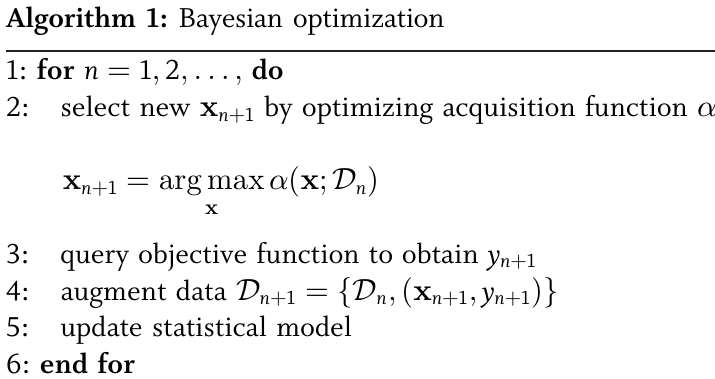
\includegraphics[width=1\textwidth]{figures/bayesian_optimization.png}
  \caption{Three steps in a Gaussian process based SMBO.}
  \label{bayesian optimization}
\end{figure}

\subsection{Aquisition Functions}
\label{aquifuncs}
The role of the aquisition function is to quantify the profitability of an objective function evaluation for a point $\x$. In the SMBO The location of the best known value of the aquisition function is the next point that will be evaluate. It is a trade off between exploitation of less known regions and exploitation of promising areas. The function described in the following can all be brought into the form:
\begin{equation}
  \alpha(\x) = \E_{y|\x}[U(\x,y)]
\end{equation}
Where $U$ is an utility function. In experiemtal design $\alpha$ is therefore also known as the expected utility.

\paragraph{Upper Confidence Bound}
An easiest way to make a tradeof beteew variance and mean is the \textit{Upper Confidence Bound}:
\begin{equation}
  \alpha_{UCB}(\x) \coloneqq \mu(\x) + \beta \cdot \sigma(\x)
\end{equation}

\paragraph{Probability of Improvement}

(Kushner 1964)

\begin{equation}
  \alpha_{PI}(\x) \coloneqq \mathbb{P}[v>\tau] = \Phi\bigg(\frac{\mu(\x)-\tau}{\sigma(\x)}\bigg)
\end{equation}

With this definition

\paragraph{Expected Improvement}
Expected Improvement (EI) was first used by Mockus et al. in 1978 \cite{mockus_application_1978} in the context of noise free computer experiments. The first application to Bayesian optimization was done by Jones in 1998 \cite{jones_efficient_1998}, who called hist approach \textit{efficient bayesian optimization}(EGO). Since empirical studies have shown good results for EI (CITATION HERE) it has become widely adopted. The utility for EI is the so called improvment function.
\begin{equation}
  \alpha_{\EI}(\x) \coloneqq \E_{y|\x}\big[(y - \tau)\mathbf{I}_{[y > \tau]}\big]
\end{equation}
With $\tau$ beening a treshold that is usually chosen as the best observed performance of the objective function $y_{max}$. $\mathbf{I}$ denotes the indicator function that equals one if $y$ is bigger than the treshold and zero if it is smaller of equal. For a Gaussian model the EI can be witten in closed form:
\begin{equation}
  \begin{split}
    \alpha_{\EI}(\x) = \int\limits_{\mathbb{R}} \max(0, y-\tau)p(y|\x)dy
    \\
    = (\mu(\x) - \tau) \cdot \Phi \bigg(\frac{\mu(\x)-\tau}{\sigma(\x)}\bigg) + \sigma \cdot \phi \bigg(\frac{\mu(\x)-\tau}{\sigma(\x)}\bigg)
  \end{split}
\end{equation}
$\phi$ is the standard normal PDF and $\Phi$ the standard normal CDF. $\mu$ and $\sigma$ are expected value and standard deviation of the model at point $\x$.
For a derivation of the closed form see appendix \ref{EI derivation}.
There are also other aquisition functions like Entropy search, which are not discussed here.

\subsection*{Aquisition optimization}
The use of a model and an aquisition function leads to a new non-convex optimization problem. The aquisition function can often be more multimodal and difficult to optimize than the original objective function. The big adavantage is the much shorter evaluation time, and hence the efficient applicability of conventional global optimization methods which often rely on numerous evaluations (but no secondary optimization problem) to find good approximative solutions.
Methods that have been applied are for example: DIRECT, L-BFGS-B, dynamic grid, ...

\subsubsection*{Recommendation Strategy}
The need for a recommendation strategy arises for noisy objective functions. In the deterministic setting the maximal aquisition value becomes the recommendation for the next evaluation step. For non-det erministic aquisition function one needs to generate a sample from a distribution over aquisition values. Strategies like returning the maximum observed value or returning the optimal latent posterior mean can be encountered. Different objective function can require different strategies \cite{hoffman_modular_2014}.

\subsection{Noisy Objective Functions}
In machine lerning experiments the objective function can be noisy, when explicite randomness is used in the algorithm or approximations of the true function are used. As described in section \ref{GPR} GPR can be defined with an additive noise term. The classical defintions of aquisiton function (section \ref{aquifuncs}) are only defined for deterministic objective functions. They heavily relay on a vanishing variance at a position once it has been observed.  In stochastic models the model variance will however converge to the noise variance ant the aquisition value never drops. SMBO algorithm would evaluate the same point ad infinitum. Redemption can come from a separate consideration of epestemic and measurment uncertainty.
EI and PI both require a threshold value $tau$ which is usually chosen as the best ever observed value of the objective function $y_{best}$. Due to noise distortion the measurment of $y_{best}$ would be underestimated.  Instead the observed filtered minimum ($\bar{y}_{best}$) can be employed, which is the minimum of the posterior averages $\mu(\x)$ of the model at every observed position $\x$.
\begin{equation}
  \bar{y}_{best} = \min_{\x \in X} \mu(\x)
\end{equation}

This approach is used in expected expected improvement (EEI) \cite{pandita_extending_2016}. The usage of EEI requires a hierachical Bayesian model with a distribution over the kernel parameters and noise variance parameter. The aquisition value is calculated by integrating over the objective function distribution (like normal EI) and over the kernel parameter distribution.

Another algorithm for stochastic BO is sequential kringing optimization (SKO) \cite{huang_global_2006}. Here EI is modified to augmented expected improvement (AEI) by multiplication with a correction term.
\begin{equation}
  \alpha_{\operatorname{AEI}} = \alpha_{\EI}(\x) \cdot \bigg(1 - \frac{\sigma_\epsilon}{\sqrt{\sigma(\x)^2 + \sigma_\epsilon^2}}\bigg)
\end{equation}
Where $\sigma_\epsilon$ denotes the noise variance and $\sigma(\x)$ (like above) the posterior varaiance of the GP-model. If the model variance is high, AEI is close to EI, but with decreasing model variance the AEI also decreases. In the way the misinterpretation of noise as epistemic uncertainty is corrected.


\subsection{Conditional Parameters}

\paragraph{The Tree-Parzen Algorithm}
The Tree-Parzen Algorithm \cite{bergstra_algorithms_2011} is a Bayesian-Optimization algorithm for tree-structured parameter spaces. Instead of modelling $p(y|\x)$ directly, $p(\x|y)$ and $p(y)$ are modelled. Instead of Gaussian processes, Gaussian-Mixture Model and Parzen-window kernel density estimation are used.

\paragraph{SMAC}
The Sequential-Model Based Algorithm Configuration \cite{hutter_sequential_2011} is used in Auto-Weka \cite{thornton_auto-weka:_2013} and Auto-Sklearn \cite{feurer_efficient_2015}. SMAC is based on Random Forrests.

\paragraph{Tree and Graph Kernels/Metrics}
An application of GPR for HPO of a deep belief network is described in \cite{bergstra_algorithms_2011}. Where multiple GP are fittet to each independent parameter groups, including the conditional groups that indicate which other goups to consider. This way they manage to use kernels that are not suitable for conditional parameter spaces out off to box. Kernels for conditional parameter spaces are developed in \cite{swersky_raiders_2014, chandar_hierarchical_2016}.

\newpage


\section{Search Space Construction}
\label{construction}
The majority of \ac{HPO} algorithms are designed for domains that are subsets of $\mathbb{R}^n$. In reality however parameter search spaces can be much more complicated. This section discribes a formalism to construct search spaces in a convenient way. First of all it must be possible to describe the parameter space of a single algorithm, which can contain an arbitrary number of integer, floating point or nominal valued parameters. Second it shall be possible to include the choice of an algorithm into the optimization process. Thrid parameters with special structure (like trees or graphs), shall also be describable in a natural way.

The first basic idea is that domains of parameters can be combined to form a new parameter space. The second idea is, that in order to express the choice between multiple algorithms, that application of algorihtms or functions must be possible. It turned out to be easier to represent both combinations and function calls as trees of application nodes.
The consequence is that the elements of a search space are not just vectors of parameter values but can be computation trees and the search space is a set of computation trees.
Since a search space can be discribed in multiple ways is must be distinguished between how a space is described and what is described. The term \textit{expression} is used to refere to the representation of a search search space. A singleton expression is called an \textit{instance}. Only instances are executable. The set of all instances that can be produced by a expression $G$ is called the \textit{extension} of $G$. The corresponding notation is a following apostrophe $G'$. While an unique extension can be assigned to every expression, an extension can be represented by multiple search spaces.

\subsection{Primitive Spaces}

Search spaces are constructed from the combination of primitive spaces. They are one dimensional collections of possible instances of a parameter.

%Every search space is ether a primitive space of a combination of primitive spaces.

\paragraph{Categorical}
Categoriacal parameters have a finite unsorted domain of numerical or non-numerical values. They are used for nominal scaled parameters, like labels in a classification problem, basis-functions in linear regression or different activation functions in feedforward neural networks.

\paragraph{Continuous}
Continues parametes are bounded or unbounded intervals over the real numbers. This type is for example used for a regularization parameter or the discount factor in Q-learning.

\paragraph{Discrete}
Values of a discrete parameters are numerical. The cardinality of a discrete parameter is finite or countable (if defined over an unbounded interval).
Other than categorical parameters, but similar to continous parameters, discrete parameters have a distance over their elements. If two elements are close, than the value of the objective fucntion is also assumed to be closed. This type is, for example, used as the number of layers in a neural network.

\subsection{Combined Spaces}
A combined space is constructed by applying operations to a series of other primitive or combined spaces. Combined search spaces can be combined again in order to create greater structures. A combined search space is represented by an application node which posseses an operation and a domain field. In programming languages, when calling a function, the arguemnts are either passed by position or passed by name. The domain field stores an objects that rembers how the paramters were applied to the operation. Mathematically this object is an indexed family. The passed-by-value arguemts are indexed by integers from $0$ to $n$ and the passed-by-name argumets are indexed by strings. This object is sometimes called a parameter list, to prevent confusion other list objects and the exsitance of keyword arguemnts, here the object is called a \textit{parameter familily}.

A parameter family with two positional arguments $A,B$ and a key keyword argument $C$ with index $x$ is written as:
$$\{A_0, B_1, C_{\text{x}}\}$$
Elements can be picked from a parameter family with the projection. It is denoted as $pi$.
$$\pi_1(\{A_0, B_1, C_\gamma\}) = B$$
Items of a parameter family can be renamed. In resemblence to relational algebra the greek letter $\rho$ is used to refer to the rename.
$$\rho_{1/a}(\{A_{0}, B_{1}\}) = \{A_{0}, B_{a}\}$$
Renaming changes the indexing of a parameter family.

\paragraph{Joining}
Two search spaces $A$ and $B$ can be joined to form a new search space, which contains all instances of $A$ and $B$. In resemblance to the Backus–Naur form, the join combination can also be expressed through a pipe symbol.
$$ \operatorname{join}(A, B) = A\ |\ B $$
The join is related to the set union, in that the extension of the join of two search spaces is the union of the extensions of these search spaces: $(A\ |\ B)' = A' \cup B'$. The only difference is that a join remembers the spaces it was constructed from.

\paragraph{Product}
The product lines up multiple search spaces to form a sequence of search spaces. It expressed by the $\prot$. If evaluated the product is evaluated it returns a parameter family.
$$\eval(\prot(A, B, C)) = \{A_0, B_1, C_2\}$$
The extension of a product of two spaces is the cartesian product of the extension of these two spaces: $\prot(A,B)' = A' \times B'$. In constrast to the cartesian product, the product of search spaces is associative.  In this way no nested structures can be constucted with the product alone. If evaluated the product returns a parameter family. Under the hood
The cartesian product of two parameter families is defined as follows. If all indices are integers the product is a usual cartesian product. The length of the first family is added to all indices of the second tuples.
$$\{A_0, B_1\} \times \{C_0, D_1\} = \{A_0, B_1, C_2, D_3\}$$
Non-integer indices are simply copied to the resulting family.
$$\{A_0,\ B_\beta\} \times \{C_0,\ D_\delta\} = \{A_0,\ C_1, B_\beta,\ D_\delta\}$$
The prodcut is undefined if two non-positional parameters share the same key.

\paragraph{Function Application}
Any function can be integrated into the system by converting it to an operation with the "op" function. If a parameter family or an expression it applied to an operation an application node is created that simply represents the application of the underlying function to the arguments. Application can be expressed with the $\apply$ function or alternatively with the $@$ operator.
$$\apply(f, A) = f\ @\ A$$
If an operation is called with multiple spaces, under the hood the product is taken of these spaces and then the operation is applied to the resulting parameter family.
$$f(A,B) = f\ @\ \prot(A,B)$$
Parameters can also be applied to joined spaces. This is equivalent the join of the correstponding function application node.
$$(f\ |\ g)(A) = f(A)\ |\ g(A)$$
With function application it finally becomes possible to express \textit{dependendencies} between parameters. Consider the joined node:
$$f(B)\ |\ g(C)$$
If $B \neq C$ then the function $f$ and $g$ have different parameter domains. The choice of the parameter is dependent on previous choice of the function.

\paragraph{Quoting}
In some cases it is required to hand an unevaluated expression to an operation. In reseblence to the correstponding operator in the Lisp programming, this is expressed by the $\operatorname{quote}$ operation. It is simply a wrapper for an expression, that returns the expression itself if evaluated: $\eval(\quot(G)) = G$.

\paragraph{Recursion}
With recursion it is possibel to express self-referential search spaces. This is done by introducting the insertion operator $<<$, which distingiushes itself from any other previous functions by its capability to change an expression, as opposed to just combining expressions to a new one. The insertion appends spaces to the parameter family of a node. In this manner expressions that have $G$ as a substructure can be inserted into $G$. Consider the following construction:
$$G \leftarrow join(A)$$
$$H \leftarrow f(G, G)$$
$$ G  \ll H$$
In the first row $G$ is initialized with a join node containing some primitve space $A$. The right arrow is the assertion operator. In the second row an application node is created, that applies $G$ to $f$ in two positions. In row three the application node is inserted into $G$. Now an expression that contains $G$ as a subexpression is a subexpression of $G$.
The extension of $G$ has infinite many elements now. If $A$ is set to a categorical space with only one element $a$, the extension looks like:
$$ G' = \{a\ ,f(a,a),\ f(a,f(a)),\ f(f(a),a),\ f(f(a),f(a)), ...\}$$
In this way the function nesting can become arbitrary deep.

\paragraph{Selection} The reverse of joining is selection. A sample from a search space can be generated by successively selecting from the joined nodes. Selection is written as $\sigma$.
$$X \leftarrow (A\ |\ B)\ |\ (C\ |\ D)$$
$$\sigma_{(1)}(X) = (C\ |\ D)$$
$$\sigma_{(0),(1)}(X) = C$$
So for nested joined nodes selection is just a path through the expression tree. To select from more complicated search space the notion of the selection shape needs to be introduced. Consider the recursive function tree $G$, from the last paragraph. The first selecetion level consists of two choices. If we select the first option $f(G,G)$, we are faced with two joined nodes with two choices each. Similar to the shape of tensors, the selection shape is a tuple that indicates the selection range of a search space.
$$\operatorname{shape}\big(G\big) = (2,)$$
$$\operatorname{shape}\big(f(G,G)\big) = (2,2)$$
$$\operatorname{shape}\big(f(G,f(G,G))\big) = (2,2,2)$$
The length of the shapes tells the number of choices that can be made at the same time. The items of the tuple are the number of options per choice. Selection from $G$ looks as follows:
$$\sigma_{(1)}(G) = f(G,G)$$
$$\sigma_{(1),(0,1)}(G) = f(A, f(G,G))$$
Figure \ref{levels} visualizes all selection options up to the third level.

\begin{figure}

  \begin{dot2tex}[tikz,options=-t math]
    digraph G {

    node [shape=box]

    b [label="f(G,G)"]
    c [label="f(A,A)"]
    d [label="f(A,f(G,G))"]
    e [label="f(f(G,G),A)"]
    f [label="f(f(G,G),f(G,G))"]

    G -> A [label="0"]
    G -> b [label="1"]
    b -> c [label="0,0", lblstyle="left=1.1cm"]
    b -> d [label="0,1"]
    b -> e [label="1,0"]
    b -> f [label="1,1"]

    }
  \end{dot2tex}


  \caption{Three selection levels of search space $G$. }
  \label{levels}
\end{figure}
Note that the extension of a selected subspace is a subset of the extension of the superspace.

$$ f(A,A)' \subset f(G,G)' \subset G' $$

\paragraph{Expression Equality}
Context free grammars can produce identical strings with a different sequence of production application. The same is true for parameter space definitions.
If a function to measure the equality of two expressions is added to the system, the search space obtains the structure of a directed acyclic graph.
Two expressions can have the same meaning even if the representations are not equal.

\paragraph{Constants \& Variables}
So far it is only possible to express search spaces over function trees.
A value that is computed once can only be used in a single other function call. With the introduction of \textit{constants} it is possible to remember the output of a computation tree evaluation. Implementationwise the constant is a wrapper around a search space, that remembers the first chosen value of that search space. Constants allow to express structures beyond the capabilities of a context free grammars. Variables are like constants, with additional ability to change value in the computation process. The elements of the search space obtain a cylic graph structures. Both constants and variables are not integrated into the system and will not be discussed further.

\subsection{Simplification}
Simplification of the search space expression can improve comprehensibility for humans, but can also improve performance of optimization algorithms applied to it. The other use of simplification is the transformation of instance expressions into a normal form, in order to detect equality of expressions.
Simplification can be realized by using methods known from term rewriting systems. In our case we can directly work on the expression, which makes simplification a mapping between expressions.
Operations can possess certain properties, which indicate the legal transformations that change the structure of the expression but maintain semantic equality.

\begin{table}[h]
\def\arraystretch{1.2}%
\centering
\begin{tabular}{c | c | l}
abbr & property name & definition \\
\hline
as               & associative        & $f(f(x,y),z) = f(x,f(y,z))$ \\
com              & commutative        & $f(x,y)=f(y,x)$ \\
ldis             & left distributive  & $f(x,g(y,z))=g(f(x,y),g(x,z))$ \\
rdis             & right distributive & $f(g(x,y),z)=g(f(x,z),g(y,z))$ \\
id               & identity           & $f(x) = x$ \\
uid              & unary idempotent   & $f(f(x)) = f(x)$ \\
bid$_{\text{1}}$ & binary idempotent  & $f(x,x) = x$ \\
bid$_{\text{2}}$ & \multicolumn{1}{|c|}{$-$} & $f(x,x) = f(x)$ \\
var              & variadic           & $f(f(x,y),z) = f(x,y,z)$\\
as/var           & \multicolumn{1}{|c|}{$-$} & $f(x,f(y,z)) = f(x,y,z)$ \\
\end{tabular}
\caption{Overview of function properties}
\label{funcprops}
\end{table}

\paragraph{commutative} Commutativity as known from binary operators indicates a symmetric realation. The order in which the arguments are applied is irrelevant. This notion can be extended to multvariate functions. The system can arbitrarily change the argument order. To bring an application of a commutative function into normal form, the parameters are sorted in alphabetical order of its serialization.

\paragraph{associative} For three or more binary associative operators in a row the application order is irrelevant. Computation trees are invariant under tree rotation if the two involved nodes are in a parent-child relationship and the operations of the node are identic and associative. For associative nodes left-to-right application conforms to the normal-form.

\paragraph{variadic}
In programming languages a variadic function is a function, that has a variable arity. Here the definition is stricter and requieres the function to be defined on an arbitrary arity ($f(),\ f(x),\ f(x_1,x_2),\ f(x_1,x_2,...,x_n)$).  The property also implies that arguments of a left-to-right applications of a node with equal operation can be merged into the parent node. An example of this is is given with the sum operation, depicted in Figure \ref{as/var transform}.

\begin{figure}

\begin{minipage}[b]{0.35\textwidth}
\caption{Two parsings of $a+b+c$. The left computation graph shows a usual left-to-right parsing, also written as sum(sum(a,b),c). With the as/var properties it can be simplified to the right computation graph sum(a,b,c).}
\label{as/var transform}
\end{minipage}%
\hfill%
\begin{minipage}[b]{0.3\textwidth}
\centering
\includegraphics[scale=0.3]{figures/sum_not_simplified.pdf}

% \label{Text}
\end{minipage}%
\hfill%
\begin{minipage}[b]{0.3\textwidth}
\centering
\includegraphics[scale=0.3]{figures/sum_simplified.pdf}
\end{minipage}%
\end{figure}

If the operation is also associative, child nodes with equal-operation can be merged into the parent node from any position (Table \ref{funcprops} row: ac/var).

\paragraph{distributive} is a property between two functions that is known from arithmetic addition and multiplication. In regard to search space expressions, function application is left and right distributive to joining.

$$f(A|B) = f(A)\ |\ f(B)$$
$$(f|g)\ @\ A = f(A)\ |\ g(A)$$
$$(f|g)\ @\ (A|B) = f(A)\ |\ f(B)\ |\ g(A)\ |\ g(B)$$

\paragraph{idempotent}
Idempotence can have different meanings. For binary operators it says that two equal operants map to the same value. For unary functions it says that the composition of this function is binary idempotent. Both are properties of the join operation. The normal form for idempotent functions is fewer function applications and fewer arguments.

\paragraph{com/as/var/bid1}
If a function is variadic, associative, commutative and binary idempotent it follows that any argument that occurs more than once can be deleted. Proof:
$$f(\alpha_1, \mathbf{x}, \alpha_2, \mathbf{x}, \alpha_3) \stackrel{com}{=}
f(\mathbf{x},\mathbf{x}, \alpha_1, \alpha_2, \alpha_3) \stackrel{as/var}{=}
f(f(\mathbf{x},\mathbf{x}), f(\alpha_1, \alpha_2, \alpha_3)) \stackrel{bid_1}{=}$$
$$f(\mathbf{x}, f(\alpha_1, \alpha_2, \alpha_3)) \stackrel{as/var}{=}
f(\mathbf{x}, \alpha_1, \alpha_2, \alpha_3)$$
The $\alpha$ variables stands for an abitrary amount of arguments. Each equal sign is labeled with the abbreviation of the property which was applied for that step (for legend see Table \ref{funcprops}).


\subsection{Structure of Search Spaces}
The range of available operations determines the possible strucutres of a search space. The search space structure again, determines the class of applicable optimizers.

Three kinds of structures need to distinguished. The \textit{instance structure} of an element of $R^n$ for example is a vector. Computation trees or matricies have a tree structure. The \textit{search space structure} (or selection structure) refres to multiple levels of choices. Conditional parameter spaces for example have a tree structure, wheres the $R^n$ is flat search space. The \textit{expression structure} is the structure of the search space representation. If a subexpression occures multiple times in an expression the expression structure becomes a directed acyclic graph, whears the search space structure remains a tree, since the choices need to be made independently.

\begin{figure}[h]
\includegraphics[scale=0.5]{figures/search_space_hierachy.pdf}
  \caption{The leftmost node represents a system with only primitive spaces. Following the edges from left to right, new operations are added. The field of a node holds the following information from top to bottom: initials of available operations, structure of search space and structure of resulting values. Constants and variables are not depicted.}
  \label{space_structure}
\end{figure}

Figure \ref{space_structure} shows the change of structure in instance and space, with the number of operations growing from left to write.
With no operations and only the primitive spaces at hand, the search space must be one dimensional and the value structure a single value.
Adding the product allows for vectors of primitives, the search space becomes multidimensional. Remember that the product is associative, which forbids nesting. The $R^n$ belongs to this structure class.
Through function application nested structes become possible, leading to tree structured instances (labeled \textbf{PA} in Figure \ref{space_structure}). All choices however remain unconditional making this the class of all flat parameter spaces.
The join operation allows the formulation of hierachical choices, and adds a tree structure to the search space. The instance structure however, remains untouched.
The class \textbf{JPA} (comprising $\join$, $\prot$ and $\apply$) is the class of conditional search spaces. The TreeParzen Algorithm is applicable to spaces form \textbf{JPA}.
With self-reference the expression structure becomes recursive. The search spaces structure becomes an infinite tree instead. Instance can become arbitrary big but not infinite.
Adding a function that test for the equality of two expressions, the search space can becomes a directed acyclic graph.
With constants once computed values can be reused an apply to multiple functions. This extends the instance structure also to directed acyclic graphs. At this point it becomes possible to express distributions over computation graphs or data flow programms.

% search space structure
% expression structure
% parameter structure



\section{Optimization of Self-Referential Seach Space}
Conventional Bayesain optimization algorithms are only suitable for flat multidimesnional search spaces or search spaces containing conditional parameters (SMAC and TreeParzen). The specification language described in the previous chapters however allows for search spaces with an arbitrary amount of parameters. The following algorithm allows to employ any Bayesian optimization model for flat parameter spaces to be applied to recursive parameter spaces.

The basic idea of the algorihm is to repetitively select subspaces from the search space until no joined node is present in the expression any more. The algorihm creates a meta tree where every node represents an expansion (selection) of the previous expression. This is similar to the depiction in figure \ref{levels}. The leaf nodes of the meta tree assigned with search space which possess only function applications and primitives. This flat subspace can be optimized locally with a conventional flat BO algorithm. The $\tau$ values used in the aquisition funciton is hereby set to the best value observed among all local optimizations.

Algorithm \ref{treebo} lists the steps form optimization in infinite-tree shaped search spaces. The root node of the meta tree is associated with the expression of the whole search space $G$. A working variable $W$ that holds the meta node of the current subexpression, is initialized with the root node (line 4). Next a full selection is chosen from $G$ by some selection criterion (see below). The meta node associatiated with this new selection is assigned to $W$ (line 6). If this selection has not been explored yet a new meta node is created (line 7). This steps are repreated until $W$ contains no join nodes any more. A leaf node is reached. The resulting search space is flat, a conventional BO-algorithm is applied to select the next evaluation point from this search space (line 11). If the result $y$ is bigger or equal that the best observer value from all other evaluations $y_{best}$, only the surrogate model associated with $W$ needs to be updated (line 17). If it is however smaller (better) than $y_{best}$ the aquisiton function for all other models change and need to be updated (line 15).

\begin{algorithm}[H]
\SetAlgoLined
initialize Root with G\;
$y_{best}$ $\leftarrow$ $\infty$\;
\Repeat{stop criterion reached}{
  W $\leftarrow$ Root\;
  \While{W is not flat}{
    W $\leftarrow$ select(W, $crit$)\;
    \If{W = null}{
      W $\leftarrow$ new node\;
    }
  }
  $\x$ = next(W)\;
  $y$ = compute($\x$)\;
  \eIf{$y$ $<$ $y_{best}$}{
    $y_{best}$ = y\;
    update all\;
  }{
    update W\;
  }
}


\caption{BO for infinite-tree structured spaces}
\label{treebo}
\end{algorithm}
%
% \While{not flat(W.search_space) }{asd}
\subsection{Selection Criteria from Subexpressions}
The selection of a subselection (algorithm \ref{treebo} line 6) was not discribed in the previous passage. Since the selection criterion for a subspace makes use of the best aquisition value of the subspace's child nodes, each nodes keeps track of this value. Once a leaf node is reached a best aquisition value arises form the underlying surrogate model. The maximal aquisition value is down propagated through the meta tree as long as it is the best value of this subexpression. If all surrogate models need to updated the aquisition values of all subtrees is also updated.

In two cases the subexpression selection is striaght forward: If a join node is completely unexplored, the selection is simply determined by random. In the other case, when all choices are sufficient explored, that an aquisition value is assigned to each child node, the subexpression with the highest value would ne chosen. Any case in between with explored and unexplored choices can be chosen by different criteria.

In the simplest approach a fix value, which servers as a default aquisition, is assigned to any unexplored node. High default aquisitions would benefit exploration of unknown structures, for self-referential expressions this leads to a faster exploration of bigger structures. Lower values would rather encourage exploration of varaints of known structures.
A more sophisticated approch is to apply \ac{GPR} on every selection level as well.

\subsection{Extention to DAG-structured Search Spaces}
As discussed in section \ref{construction} the structural equality of subexpressions or semantic equality of different instances, turns the search space into a directed acyclic graph. In this case the expression meta tree also turns into DAG. Basically all update steps stay the same, with the exeption of the creation of new meta nodes. If an unexplored subexpression matches the expression of another meta node the pointer gets assigned to this node instead.

\subsection{Parallelization}
A sequential Bayesian Optimization Algorithm can be extended to parrallel Algorithm with one simple trick. If an evaluation point is chosen, instead of waiting for the actual result, the expeced value estimate, which is easilz exessible with the Gaussian model, is inserted as a placeholder. The selection process is initiated again and will chose another point since the variance of the former point is zero. One the computation is complete the placeholder value is substituted by the real value. In this way objective function evaluations can be parralelized, while parameter selection keeps sequential.

\subsection{Integration with Manual Search}
Manual guidance before and during the optimization process.

\subsubsection*{Prior Information}
In machine learning preknowledge about the learning task can be consindered as choice and distribution over the hypothesis space. This is determined rather indirect by the choice of the \ac{ML}-algorithm and its hyperparameters (or distribution over hyperparameters) or in Bayesian method directly expressed via prior probabilities. Since gaussian processes regession is used here, the choice of the kernel
Prior infotmation can for example be an actual probabilistic prior over the search space. For random sampling this probability can just be used as the sampling probability. For model-based methods, which have no direct sampling, this probability can be interpreted as \textit{probability of improvement} or (more plausible) as \textit{probability of optimum}.

\subsubsection*{Search Hints}
A concept I labeled \textit{search hints} is a way to express external knowledge about the search space. I contranst to regular prior knowledge search hits can also be injected into search process on the fly. Intuitively a search hint just denotes good region to search. And once again it is not obvious how to translate this human instructions into the search process.
The easier part is to construct a probability distribution only from hints. If a hint is interpreted as a sample from the space of the probability of optimum then distribution estimation methods like Parzen-Window can be used. If one takes a squard exponential kernel, a hint translates to good region. To indicate better regions one would need to give multiple of samples from the same region, which is unfavourable. To solve this one could give weighted hints. Once again there are different ways to do this.
First one could assign the probability of optimium directly to a region. This however is hard to conceptualize for users and requires not to violate the normalization property (sum of hints must not excede one).
A second way is to allow values between zero and one, fit a curve, and normlize aferwards to get a probability of optimum. Which is much better, because a value of zero keeps the interpretation of zero probability and one get the interpretation of maximum probability. If one allows arbitrary big values for hints the down scaling of former hints could become easier. If one allows also negative values, and includes adding the absolute value of the smalles negative value to all hints, upscaling of former hints would become possible. In both extensions however one looses the interpretation of one and zero.
The third method interpretes hints as a modification of an already existing model.
In an active learning setting point hints can be handeled without an model modification, by simply forcing this hints into the processing queue.

intuitive way to do this is ascribing an increase in probability to positive hints and and decrease in probability to negative hints.


\subsection{Objective Function Approximation}


\section{Implementation}
The formalism is implemented as a package for the programming language Python. The code repository can be accessed on \url{http://github.com/mome/baumschule}. For Gaussian processe regression the implementation relies on the GPy library \footnote{\url{http://github.com/SheffieldML/GPy}}.

Primitive spaces can be constructed by using the \python{convert} function. Python sets are converted to categorical and lists to discrete sapces. Dictionaries (with keyes of type \python{str} or \python{int}) are converted to product nodes. Continous parameters can be constructed by slicing from real numbers. For example floating point values from -1 to 3.5 are written with \python{R[-1:3.5]}. Internally \python{R} is represented as an open intervall from minus infinity to plus infinity. Discrete parameterers can be constructed in the same way by slicing from \python{N}. Create a joined node with \python{join} or the pipe operator (\python{|}). Create a product node with \python{prod}. Insertion can be done with the left shift operator (\python{<<}). There is support for arithmetics with builtin operations (\python{add}, \python{sub}, \python{mul} and \python{div}) or simply by using the correstponding python operators on two parameterspaces (\python{+}, \python{-}, \python{*} and \python{/}). Parameter families can be converted to python containers with the operations: \python{list_op}, \python{tuple_op}, \python{dict_op} and \python{set_op}.
The \python{operation} function (short \python{op}) creates an operation from a python function. Operation objects are callable, so application is expressed with normal calling notation. Alternatively the \python{apply} operation or the @-operator does the same thing. The \python{minimize_func} function takes an objective function, a parameter space, a stopping criterium and a string to specify the opimizer.  The currently implemented optimizers are random search, Bayesian Optimization for unconditional spaces and Bayesian Optimization for infinte tree structured spaces. The \python{"minimize_func"} function returns a minimization object, which is executed with \python{.run()} or can be run in a separate thread with \python{.start()}. A minimization object has a dict of observers that get notified about all executions and results. The \python{"standard"} observer stores a list of tuples with instance, start/finsh times and results.
For better inspection an expression can be rendered as a graph using the Python bindings for "Graphviz". The \python{to_dot} function returns an graph objects that can be stored to an image file, or will be displayed in an IPython Notebook or QtConsole automatically. All visualizations of expressions have been rendered with \python{to_dot}.

\paragraph{Sampling} Search spaces have a \python{.dist} field that stores a probability distribution over the domain. The \python{sample} function uses this distribution to sample instancse from an expression. It is for example used for random search and the first two steps in Bayesian Optimization. Samping starts at the root. If the node is a joined, one element of the domain gets chosen. The sample function is then applied on the chosen element recursively until the current node is primitive. For other application nodes, sample is applied to every member of the parameter family. If no distribution is assigned, a default distribution is used instead. Table \ref{default dists} shows the default distributions for each parameter type. This behavior can be changed in the configuration. A sampled instance can be evaluated with the \python{compute} function.

\begin{table}
\centering
\begin{tabular}{|l|l|}
\hline joined & discrete uniform \\
\hline categorical & discrete uniform \\
\hline bounded discrete & discrete uniform \\
\hline one sided unbounded discrete & ? \\
\hline two sided unbounded discrete & ? \\
\hline bounded continuous & continous uniform \\
\hline one sided unbounded continuous & truncated standard normal \\
\hline two sided unbounded continuous & standard normal \\
\hline
\end{tabular}
\caption{Default distributions.}
\label{default dists}
\end{table}


\subsection{Examples}

\paragraph{Minimum of two functions}
\begin{minted}{python}
from baumschule import *

# declare objective fucntions
@operation
def f(x, y):
    return x**2 + y**2

@operation
def g(x):
    return x**2 + 1

# declare parameter search space
fss = f(
    x = R[-10:10],
    y = R[:10],
)
gss = g(R)
search_space = join(fss, gss)

# minimize function wit 100 iterations
min_obj = minimize(search_space, max_iter=100)
min_obj.run()

\end{minted}

\paragraph{Kernel Grammar}

\begin{minted}{python}
import numpy as np
import GPy
from baumschule import *

# Bayesian information criterion of a GPy model
def bic(model):
    return -2 * model.log_likelihood() + np.log(len(model.X)) * model.size

kernel_dict = {
    'RBF' : GPy.kern.RBF,
    'EXP' : GPy.kern.Exponential,
    'BIAS': GPy.kern.Bias,
    'LINEAR' : GPy.kern.Linear,
}

# construct search space
K = convert(set(kernel_dict.keys()))
K.symbol = 'K'
K = op(kernel_dict.get)(K)(1)
G = join()
G << (K+G | K*G | K)
G = simplify(G)

# load data
data = load('01-airline.mat')
x_train = data['X']
y_train = data['y']

# define objective function
def objective(kernel):
    m = GPy.models.GPRegression(x_train, y_train, kernel)
    m.optimize()
    return bic(m)

# create and run optimization
opt_obj = minimize_func(objective, G, max_iter=100)
opt_obj.run()

\end{minted}


\paragraph{Multilayer Perceptron, with variable layers}
The ...


\begin{minted}{python}
from baumschule import *
from sklearn.neural_network import MLPClassifier
from sklearn.datasets import fetch_mldata
from sklearn.model_selection import train_test_split

mnist = fetch_mldata('MNIST original', data_home='~/data/baumschule')

X_train, X_test, y_train, y_test = train_test_split(
     mnist.data, mnist.target, test_size=0.4)

@operation
def train_and_validate(model):
    model.fit(X_train, y_train)
    score = model.score(X_test, y_test)
    error = -1 * score + 1
    return error

# define grammar for network layers:
# abitrary length tuple, with integrers between 1 and 100
nn = N[:100]
layers = join()
layers << (prod(nn, layers) | nn)
layers = tuple_op(layers) # converts parameter family to tuple
layers = simplify(layers) # merges the join nodes

# set parameters of classifier
parameters = convert({
    'hidden_layer_sizes' : layers,
    'activation' : {'identity', 'logistic', 'tanh', 'relu'},
    'learning_rate' :  {'constant', 'invscaling', 'adaptive'},
})

# apply paramters to classifier and model to validation routine
model_space = op(MLPClassifier)(parameters)
search_space = train_and_validate(model_space)

# run optimization and save results
min_obj = minimize(search_space, max_iter=100)
min_obj.run()
min_obj.observers['standard'].to_csv('mnist_mlp.csv')

\end{minted}

\begin{figure}
  \includegraphics[width=1\textwidth]{figures/mlp_search_space.pdf}
  \caption{Visualization produced by the "to\_dot" function, showing the search space of the multilayer perceptron. Red nodes are primitive, blue nodes are application, yellow means combination.}
  \label{mlp_search_space}
\end{figure}


\section{Experiments}
A first experiment of unconditional BO on vaious multimodal objective function with a domain from $\mathbb{R}^n$, clearly showed a better performance for BO compared to random search. A variation in aquisition function showed no signifficant effect.

\subsection{Gaussian Process Regression}
\paragraph{Kernel Combination Optimization}
\paragraph{Kernel Parameter and Kernel Combination Optimization}
\subsection{Elastic Net Linear Regression}
\subsection{Feat-Forward Networks}
\subsection{Self Optimization}

\section{Conclusion \& Outlook}
...

\begin{enumerate}
  \item{Connection to Functional Programming}
  \item{Connection to Constraint Satisfaction Problems}
  \item{Connection to Probabilistic Programming}
  \item{Connection to Reinforcement Learning}
  \item{Integration with Workflow-Managers}
\end{enumerate}



\appendix

\section{Derivation of Expected Improvement}
\label{EI derivation}
I counld not find derivation of the closed-form version of expected improvement anywhere in the litterature, so I just add it here. Note that for simplicity $\mu(\x)$ and $\sigma(\x)$ have been replaced with $\mu$ and $\sigma$.

$$\alpha_{\EI}(\x) := \mathbb{E}_{y|\x}[max(y-\tau, 0)]\ $$

$$= \int\limits_{\tau}^{\infty}(x-\tau)dp(y|\x) = \int\limits_{\tau}^{\infty}(x-\tau)\mathcal{N}(y;\mu,\sigma)dy$$

$$ = \frac{1}{\sigma\sqrt{2\pi}} \int\limits_{\tau}^{\infty}(y-\tau)e^{-\frac{1}{2}\big(\frac{y-\mu}{\sigma}\big)^2}dy =
\frac{1}{\sqrt{2\pi}} \int\limits_{(\tau-\mu)/\sigma}^{\infty}(u\sigma+\mu-\tau)e^{-\frac{1}{2}u^2}du$$

$$=\frac{1}{\sqrt{2\pi}}\bigg((\mu-\tau) \mkern-12mu \int\limits_{(\tau-\mu)/\sigma}^{\infty} \mkern-10mu e^{-\frac{1}{2}u^2}du + \sigma \mkern-12mu \int\limits_{(\tau-\mu)/\sigma}^{\infty} \mkern-10mu u e^{-\frac{1}{2}u^2}du \bigg)$$

$$=(\mu-\tau)\bigg|\ \Phi(u)\ \bigg|_{(\tau-\mu)/\sigma}^{\infty} \mkern-6mu + \ \ \ \sigma\bigg|-\frac{1}{\sqrt{2\pi}}e^{-\frac{1}{2}u^2}\bigg|_{(\tau-\mu)/\sigma}^{\infty}$$

$$=(\mu-\tau)\bigg(1-\Phi\bigg(\frac{\tau-\mu}{\sigma}\bigg)\bigg) + \sigma \cdot \phi \bigg(\frac{\tau-\mu}{\sigma}\bigg)$$

$$ = (\mu - \tau) \cdot \Phi \bigg(\frac{\mu-\tau}{\sigma}\bigg) + \sigma \cdot \phi \bigg(\frac{\mu-\tau}{\sigma}\bigg)$$


\section{Formal descriptions}
Join and prod over parameter-lists form an idempotent semiring:

$(A, \cup)$ is a idempotent commutative monoid (or join-semilatice with zero) with identity element $\emptyset$:
$$(a \cup b) \cup c = a \cup (b \cup c)$$
$$\emptyset \cup a = a \cup \emptyset = a$$
$$a \cup b = b \cup a$$
$$a \cup a = a$$

$(A, \times)$ is a commutative monoid with identity element $[\ ]$:
$$(a \times b) \times c = a \times (b \times c)$$
$$[\ ] \cup a = a \cup [\ ] = a$$

Product left and right distributes over join:
$$a\times(b \cup c) = (a\times b) \cup (a\times c)$$
$$(a \cup b)\times c = (a\times c) \cup (b\times c)$$

Product by $\emptyset$ annihilates $A$:
$$\emptyset \times a = a \times \emptyset = \emptyset$$


\printbibliography


 \end{document}
